%% SoftwareX -- Original Software Publication
%% Built on Elsevier's elsarticle class (a copy is shipped in this folder).
\documentclass[preprint,12pt]{elsarticle}

\usepackage{amsmath,amssymb}
\usepackage{graphicx}
\usepackage{booktabs}
\usepackage{array}
\usepackage{tikz}
\usetikzlibrary{arrows.meta,positioning,fit,calc}
\usepackage{listings}
\usepackage{xcolor}
\usepackage[hidelinks]{hyperref}
\usepackage{lineno}

\graphicspath{{../figures/verification/}}

\lstset{basicstyle=\ttfamily\small, columns=fullflexible, keepspaces=true,
  frame=single, rulecolor=\color{black!30}, xleftmargin=4pt, xrightmargin=4pt,
  aboveskip=6pt, belowskip=6pt, showstringspaces=false,
  keywordstyle=\color{blue!60!black}, commentstyle=\color{black!55},
  language=Python}

\journal{SoftwareX}
\emergencystretch=1.5em
\providecommand{\doi}[1]{\href{https://doi.org/#1}{doi:\nolinkurl{#1}}}

\begin{document}

\begin{frontmatter}

\title{PlasmaWaveLab: A verified Python package for Sagdeev pseudopotential
analysis and spectral Korteweg--de Vries simulation of ion-acoustic solitary waves}

\author{Alvaro H. Salas\corref{cor1}}
\ead{ahsalass@unal.edu.co}
\cortext[cor1]{Corresponding author. ORCID: 0000-0001-9343-6062}
\address{FIZMAKO Research Group, Department of Mathematics and Statistics,
Universidad Nacional de Colombia, Sede Manizales, Manizales, Colombia}

\begin{abstract}
PlasmaWaveLab is an open-source Python package for the reproducible computation
of one-dimensional electrostatic ion-acoustic solitary waves at two levels of
description. A Sagdeev module treats the fully nonlinear cold-ion/Boltzmann-electron
fluid--Poisson model: it evaluates the pseudopotential, determines the critical
Mach number $M_c\simeq1.5852$, locates the soliton amplitude by bracketed root
finding and reconstructs the spatial profile. A Korteweg--de Vries (KdV) module
evolves the weakly nonlinear limit of the same model on a periodic domain with a
de-aliased Fourier pseudospectral discretisation and a fourth-order
integrating-factor Runge--Kutta scheme. The two modules are linked through the
explicit small-amplitude mapping $\phi_m\to3(M-1)$, which the package verifies
numerically. A single script regenerates every figure and number in this paper,
including spectral convergence in space, observed fourth-order convergence in
time, first-order agreement with the KdV limit, agreement with the exact
two-soliton phase shifts, mass conservation to round-off and a relative drift
of the other invariants of order $10^{-10}$ over $2\times10^4$ time steps. The package is intended as a transparent,
tested reference for teaching, for verifying more elaborate plasma-wave codes,
and as a base for extensions to multi-species plasmas.
\end{abstract}

\begin{keyword}
Sagdeev pseudopotential \sep ion-acoustic solitons \sep Korteweg--de Vries equation
\sep Fourier spectral method \sep code verification \sep Python
\end{keyword}

\end{frontmatter}

%% ------------------------------------------------------------------
\section*{Code metadata}
\label{sec:metadata}

\begin{table}[h!]
\centering\small
\begin{tabular}{|p{0.7cm}|p{5.3cm}|p{6.2cm}|}
\hline
\textbf{Nr.} & \textbf{Code metadata description} & \textbf{Metadata} \\
\hline
C1 & Current code version & v0.3.0 \\
\hline
C2 & Permanent link to code/repository used for this code version &
\url{https://github.com/alvarohumberto/PlasmaWaveLab} \\
\hline
C3 & Permanent link to reproducible capsule & Not applicable;
\texttt{examples/verification.py} reproduces all results \\
\hline
C4 & Legal code license & MIT License \\
\hline
C5 & Code versioning system used & git \\
\hline
C6 & Software code languages, tools and services used & Python; NumPy, SciPy,
Matplotlib; pytest; GitHub Actions \\
\hline
C7 & Compilation requirements, operating environments and dependencies &
Python $\geq$ 3.10 on Linux, macOS or Windows; \texttt{numpy>=1.24},
\texttt{scipy>=1.10}, \texttt{matplotlib>=3.7}; no compilation required \\
\hline
C8 & If available, link to developer documentation/manual &
\url{https://github.com/alvarohumberto/PlasmaWaveLab/tree/main/docs} \\
\hline
C9 & Support email for questions & \href{mailto:ahsalass@unal.edu.co}{ahsalass@unal.edu.co} \\
\hline
\end{tabular}
\caption{Code metadata.}
\label{tab:metadata}
\end{table}

\linenumbers

%% ------------------------------------------------------------------
\section{Motivation and significance}
\label{sec:motivation}

Ion-acoustic solitary waves are the canonical example of coherent nonlinear
structures in plasmas. They were predicted theoretically in the 1960s
\cite{Sagdeev1966,WashimiTaniuti1966}, observed in the laboratory shortly
afterwards \cite{Ikezi1970}, and remain a standard topic in plasma courses
\cite{Chen2016}. Two complementary descriptions are used. Sagdeev's
pseudopotential method \cite{Sagdeev1966} treats stationary travelling waves of
the fully nonlinear fluid--Poisson system and reduces the existence question to
the motion of a pseudo-particle in a potential well. Reductive perturbation
theory \cite{WashimiTaniuti1966} yields instead the Korteweg--de Vries (KdV)
equation \cite{Korteweg1895}, which describes the time evolution, interaction and
stability of small-amplitude waves \cite{ZabuskyKruskal1965,DrazinJohnson1989}.

In the research literature, both kinds of calculation are usually carried out
with short, unpublished scripts. Root brackets, integration tolerances, tail
truncation, grid resolution and time step are rarely reported, so
published amplitudes, existence domains and profiles are difficult to reproduce
or to compare between papers. The difficulty is compounded in extensions to
multi-species, dusty or non-thermal plasmas, where the new results have no
independent reference. General-purpose spectral frameworks such as Dedalus
\cite{Burns2020} can integrate the KdV equation, but they do not address the
Sagdeev problem and are heavier than needed for verification and teaching.

PlasmaWaveLab fills this gap with a small, fully tested, documented package that
(i) solves the Sagdeev problem for the cold-ion/Boltzmann-electron plasma,
including the critical Mach number; (ii) integrates the corresponding KdV
equation with a spectrally accurate, fourth-order time-stepping method; and
(iii) connects the two descriptions through their explicit asymptotic relation,
so that each module serves as an independent check of the other. The main
numerical parameters are function arguments with documented defaults, and one
script reproduces every figure and number in this article
(Section~\ref{sec:examples}).

%% ------------------------------------------------------------------
\section{Software description}
\label{sec:description}

\subsection{Mathematical models}
\label{sec:models}

All quantities are dimensionless: the potential $\phi$ is normalised by
$k_BT_e/e$, lengths by the electron Debye length, velocities by the
ion-acoustic speed $c_s$, and densities by the equilibrium density. For cold
ions and Boltzmann electrons, a wave travelling at Mach number $M$ with
coordinate $\xi=x-Mt$ satisfies the energy integral
\begin{equation}
\frac12\left(\frac{\mathrm d\phi}{\mathrm d\xi}\right)^2+S(\phi;M)=0,\qquad
S(\phi;M)=1-e^{\phi}+M^2\left(1-\sqrt{1-\frac{2\phi}{M^2}}\right),
\label{eq:sagdeev}
\end{equation}
which is real only for $\phi<M^2/2$ \cite{Sagdeev1966,Chen2016}. A
positive-polarity soliton of amplitude $\phi_m$ exists when $S(\phi_m;M)=0$
with $S<0$ on $(0,\phi_m)$. Since $S''(0)=M^{-2}-1$, this requires $M>1$, and the
root must lie below the ion-density limit, which gives the upper bound
\begin{equation}
1-e^{M_c^2/2}+M_c^2=0\quad\Longrightarrow\quad M_c\simeq1.5852 .
\label{eq:mc}
\end{equation}

Setting $M=1+\delta$ with $0<\delta\ll1$ and expanding (\ref{eq:sagdeev}) gives
$S\simeq-\delta\phi^2+\phi^3/3$, whose solution is
$\phi\simeq3\delta\,\mathrm{sech}^2(\sqrt{\delta/2}\,\xi)$. This is exactly the
soliton of
\begin{equation}
u_t+\alpha\,u\,u_x+\beta\,u_{xxx}=0,\qquad
u_{\rm sol}=A\,\mathrm{sech}^2\!\left[\sqrt{\tfrac{\alpha A}{12\beta}}
\left(x-x_0-\tfrac{\alpha A}{3}t\right)\right],
\label{eq:kdv}
\end{equation}
with $\alpha=1$, $\beta=1/2$, $A=3\delta$ and speed $\delta=M-1$ in the
frame moving at $c_s$, which is the ion-acoustic KdV equation of Washimi and
Taniuti \cite{WashimiTaniuti1966}. The KdV module accepts arbitrary positive
$\alpha,\beta$, so it also covers other plasmas whose reduction leads to
(\ref{eq:kdv}). The function \texttt{ion\_acoustic\_kdv\_coefficients()} returns
the values for the present model.

\subsection{Numerical methods}
\label{sec:numerics}

\emph{Sagdeev module.} Values $M\le1$ are rejected immediately. Otherwise the
amplitude $\phi_m$ is bracketed by sampling $S$ at 2500 points just below the
ion-density limit $M^2/2$, identifying the last negative sample followed by a
positive one, and refining with Brent's method \cite{Brent1973} to an absolute
tolerance of $10^{-13}$. If no such sign change exists ($M\ge M_c$), a
descriptive exception is raised instead of returning a spurious branch. The profile is
obtained by integrating $\phi''=-S'(\phi;M)$ from the crest
$(\phi,\phi')=(\phi_m,0)$ with an adaptive Dormand--Prince scheme
\cite{DormandPrince1980} (relative and absolute tolerances
$2\times10^{-10}$ and $2\times10^{-12}$). The origin is a saddle point of this
system, so the trajectory is terminated when $\phi$ falls to $10^{-5}\phi_m$,
and the profile is set to zero beyond that point and mirrored about the crest.

\emph{KdV module.} Equation~(\ref{eq:kdv}) is discretised on a periodic grid of
$N$ points with Fourier differentiation \cite{FornbergWhitham1978,Trefethen2000}.
In Fourier space $\hat u_t=L\hat u+\hat N(\hat u)$ with $L_k=i\beta k^3$ and
$\hat N_k=-\tfrac{i}{2}\alpha k\,\widehat{u^2}$, where the quadratic product is
filtered with a two-thirds wavenumber mask to suppress aliasing \cite{Orszag1971}. The stiff linear part is
integrated exactly by an integrating factor, and the remaining system is advanced
with the classical fourth-order Runge--Kutta method (IF-RK4) \cite{Trefethen2000}.
Exponential time-differencing alternatives are discussed in
\cite{CoxMatthews2002,KassamTrefethen2005}. The mass
$\int u\,dx$, the $L^2$ norm $\int u^2dx$ and the Hamiltonian
$\int(\beta u_x^2/2-\alpha u^3/6)\,dx$ are evaluated spectrally as diagnostics.

\subsection{Software architecture}
\label{sec:architecture}

The package follows a standard \texttt{src}-layout (Fig.~\ref{fig:arch}). All
numerical routines live in \texttt{core.py} as pure functions of NumPy arrays
and scalars, without global state, so they can be called from scripts, notebooks
or other packages. The command-line interface (\texttt{\_\_main\_\_.py}) is a
thin layer that parses parameters, calls the core functions and writes PNG
figures and CSV tables. The script \texttt{examples/verification.py} produces
all results in Section~\ref{sec:examples} and writes them to CSV files and a
machine-readable \texttt{summary.json}, which records the versions of Python, NumPy, SciPy and
Matplotlib and the platform. The package builds on NumPy \cite{Harris2020}, SciPy
\cite{Virtanen2020} and Matplotlib \cite{Hunter2007}. The test suite (21 tests) checks analytical derivatives, the critical
Mach number, the small-amplitude limit, spatial and temporal convergence rates,
invariant drift, input validation and the command-line interface. It runs on
Python 3.10--3.13 through GitHub Actions on every push.

\begin{figure}[t]
\centering
\resizebox{0.92\linewidth}{!}{%
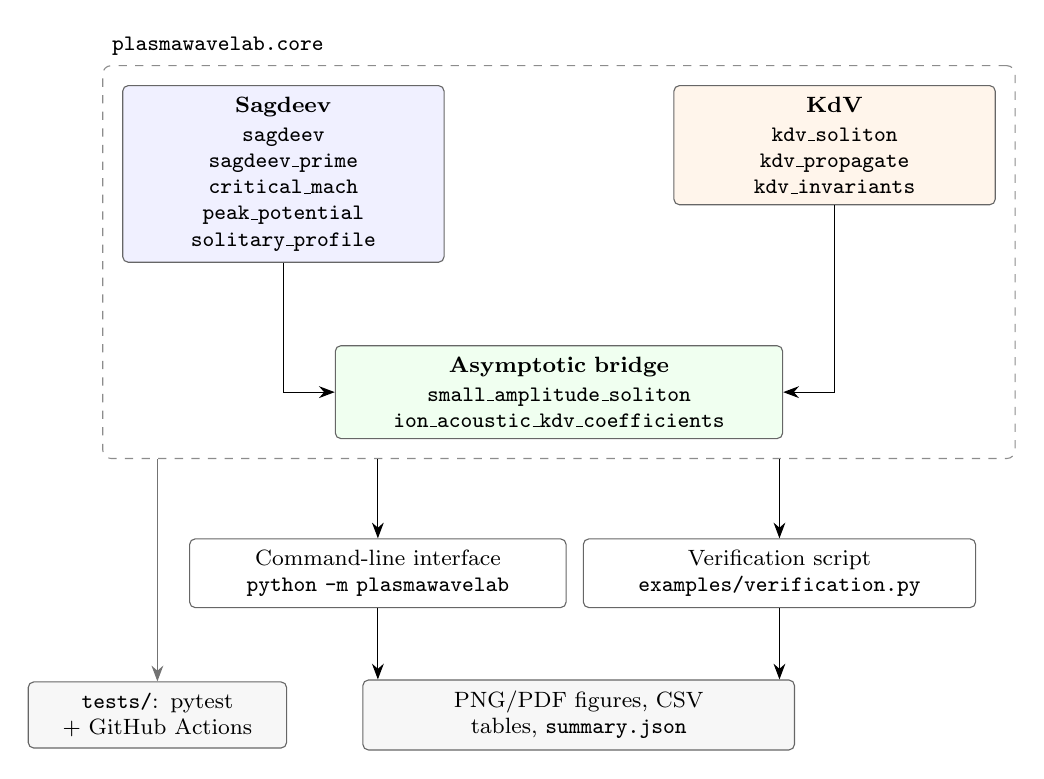
\begin{tikzpicture}[font=\footnotesize, >={Stealth[length=2mm]},
  box/.style={draw=black!60, rounded corners=2pt, align=center, inner sep=4pt,
              text width=#1}, box/.default=3.6cm]
\node[box=3.8cm, fill=blue!6, anchor=north]   (sag) at (0,0) {\textbf{Sagdeev}\\[1pt]
  \texttt{sagdeev}\\ \texttt{sagdeev\_prime}\\ \texttt{critical\_mach}\\
  \texttt{peak\_potential}\\ \texttt{solitary\_profile}};
\node[box=3.8cm, fill=orange!8, anchor=north] (kdv) at (7,0) {\textbf{KdV}\\[1pt]
  \texttt{kdv\_soliton}\\ \texttt{kdv\_propagate}\\ \texttt{kdv\_invariants}};
\node[box=5.4cm, fill=green!6]  (bri) at (3.5,-3.9) {\textbf{Asymptotic bridge}\\[1pt]
  \texttt{small\_amplitude\_soliton}\\ \texttt{ion\_acoustic\_kdv\_coefficients}};
\draw[->] (sag.south) |- (bri.west);
\draw[->] (kdv.south) |- (bri.east);
\node[draw=black!45, dashed, rounded corners=3pt, inner sep=7pt,
      fit=(sag)(kdv)(bri)] (core) {};
\node[anchor=south west, font=\footnotesize\ttfamily] at (core.north west) {plasmawavelab.core};
\node[box=4.5cm] (cli) at (1.2,-6.2) {Command-line interface\\ \texttt{python -m plasmawavelab}};
\node[box=4.7cm] (ver) at (6.3,-6.2) {Verification script\\ \texttt{examples/verification.py}};
\node[box=5.2cm, fill=black!3] (out) at (3.75,-8.0) {PNG/PDF figures, CSV tables, \texttt{summary.json}};
\node[box=3.0cm, fill=black!3] (tst) at (-1.6,-8.0) {\texttt{tests/}: pytest\\ + GitHub Actions};
\draw[->] (cli.north |- core.south) -- (cli.north);
\draw[->] (ver.north |- core.south) -- (ver.north);
\draw[->] (cli.south) -- (cli.south |- out.north);
\draw[->] (ver.south) -- (ver.south |- out.north);
\draw[->, black!55] (tst.north |- core.south) -- (tst.north);
\end{tikzpicture}}
\caption{Architecture of PlasmaWaveLab. The core module holds the two solvers
and the asymptotic bridge between them. The command-line interface, the
verification script and the test suite are thin clients of the core.}
\label{fig:arch}
\end{figure}

\subsection{Software functionalities}
\label{sec:functionalities}

\begin{itemize}
\item Evaluation of $S(\phi;M)$ and $S'(\phi;M)$, with checks on the domain
  of definition.
\item Computation of $M_c$ and of the soliton amplitude $\phi_m(M)$ for
  $1<M<M_c$, with descriptive errors outside this range.
\item Reconstruction of the symmetric soliton profile $\phi(\xi)$.
\item The leading-order KdV approximation of the Sagdeev soliton and the
  corresponding $(\alpha,\beta)$ coefficients.
\item Exact KdV solitons for arbitrary $(A,\alpha,\beta,x_0)$.
\item Periodic KdV evolution of arbitrary initial data with user-selected $N$,
  domain length, $\Delta t$, final time and snapshot interval.
\item Spectral evaluation of mass, $L^2$ norm and Hamiltonian.
\item Command-line access to all of the above, with CSV and PNG output for use
  outside Python.
\end{itemize}

\subsection{Sample code snippet}
\label{sec:snippet}

\begin{lstlisting}
import numpy as np
import plasmawavelab as pwl

pwl.critical_mach()                 # 1.5852010652...
phi_m = pwl.peak_potential(1.2)     # 0.5243854849...
xi, phi, amp, xi_end = pwl.solitary_profile(1.2)

# Two-soliton collision on a periodic domain
L, N = 150.0, 512
x = np.linspace(-L/2, L/2, N, endpoint=False)
u0 = (pwl.kdv_soliton(x, 0, amplitude=2.0, center=-50)
      + pwl.kdv_soliton(x, 0, amplitude=0.5, center=-25))
t, U = pwl.kdv_propagate(u0, length=L, final_time=100, dt=0.005)
pwl.kdv_invariants(U[-1], L/N)      # mass, l2, hamiltonian
\end{lstlisting}

The same computations are available from the shell, for example:
\begin{lstlisting}[language=bash]
plasmawavelab sagdeev --mach 1.2 --output results/sagdeev
plasmawavelab kdv --n 512 --time 2 --alpha 1 --beta 0.5
\end{lstlisting}

%% ------------------------------------------------------------------
\section{Illustrative examples}
\label{sec:examples}

All results below were produced by \texttt{python examples/verification.py}
with PlasmaWaveLab 0.3.0, Python 3.13, NumPy 2.5 and SciPy 1.18 on a single core
of an Intel Xeon (2.8\,GHz) Linux virtual machine (as recorded in
\texttt{summary.json}). The complete script runs in
about 12\,s. The numbers quoted are read from the generated
\texttt{summary.json} file, and Table~\ref{tab:verification} summarises them.

\paragraph{Sagdeev solitons and existence domain}
Fig.~\ref{fig:sagdeev}a shows the pseudopotential for four Mach numbers across
the existence domain, and Fig.~\ref{fig:sagdeev}b the corresponding profiles.
As $M$ increases, the well deepens and the soliton becomes taller and narrower.
For $M=1.2$ the computed amplitude is $\phi_m=0.524385485$. Fig.~\ref{fig:existence}a
traces $\phi_m(M)$ over the whole branch. The curve meets the ion-density bound
$M^2/2$ at $M_c=1.585201065$, in agreement with Eq.~(\ref{eq:mc}). For
$M>M_c$ the package reports that no soliton exists.

\begin{figure}[t]
\centering
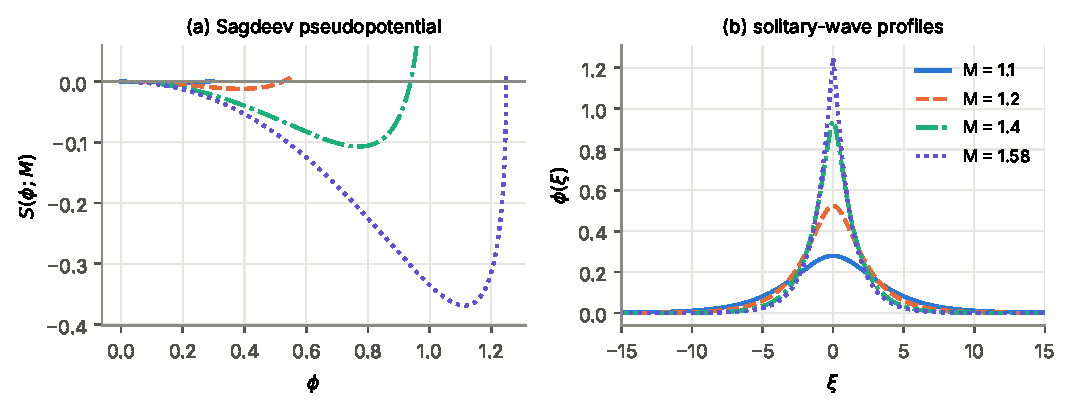
\includegraphics[width=\linewidth]{fig_sagdeev.pdf}
\caption{(a) Sagdeev pseudopotential $S(\phi;M)$ and (b) reconstructed
solitary-wave profiles for $M=1.1$, $1.2$, $1.4$ and $1.58$.}
\label{fig:sagdeev}
\end{figure}

\paragraph{Agreement between the two models}
The KdV limit provides an independent check of the Sagdeev solver.
Fig.~\ref{fig:existence}b shows the relative difference between the computed
soliton and $3\delta\,\mathrm{sech}^2(\sqrt{\delta/2}\,\xi)$ for
$\delta=M-1$ between $0.005$ and $0.16$. Both the amplitude error and the
maximum-norm profile error decrease linearly with $\delta$ (fitted slope 0.96).
This is the expected first-order behaviour of the next term of the asymptotic
expansion: the profile error is $0.64\%$ at $\delta=0.005$ and $17.8\%$ at
$\delta=0.16$. The comparison also shows the user quantitatively where the KdV
description breaks down.

\begin{figure}[t]
\centering
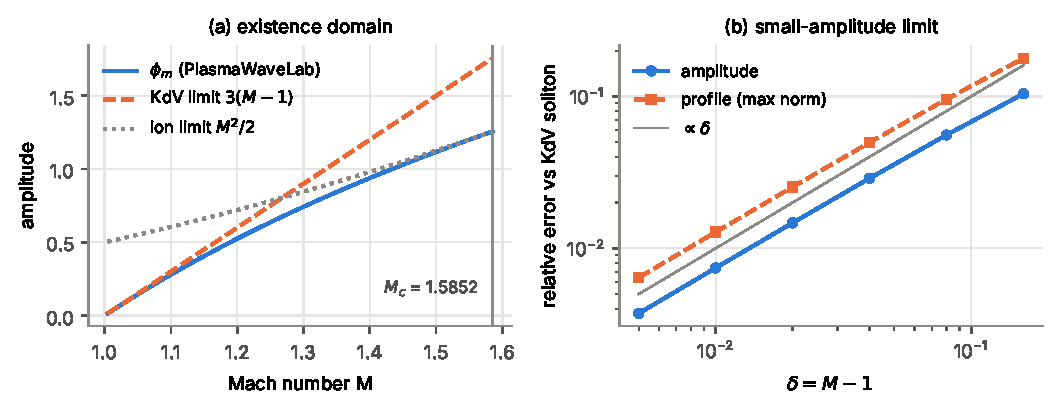
\includegraphics[width=\linewidth]{fig_existence.pdf}
\caption{(a) Soliton amplitude over the existence domain $1<M<M_c$, compared
with the KdV limit $3(M-1)$ and the ion-density bound $M^2/2$. (b) Relative
difference between the fully nonlinear Sagdeev soliton and its KdV
approximation as a function of $\delta=M-1$.}
\label{fig:existence}
\end{figure}

\paragraph{Convergence of the KdV solver}
A single soliton ($A=1$, $\alpha=\beta=1$, $L=120$) propagated to $t=2$
converges spectrally in $N$ (Fig.~\ref{fig:convergence}a). The maximum error
decreases from $7.5\times10^{-2}$ at $N=48$ to $7.6\times10^{-10}$ at $N=256$
and $2.2\times10^{-14}$ at $N=384$, which is round-off level. With a resolved grid
($N=512$, $A=2$, $t=4$), the temporal error
(Fig.~\ref{fig:convergence}b) decreases from $3.8\times10^{-5}$ at $\Delta t=0.08$ to
$2.8\times10^{-10}$ at $\Delta t=0.005$. Apart from the coarsest, pre-asymptotic
step (apparent order 5.1), the observed orders between successive refinements
are 3.90, 3.97 and 3.99, which confirms the design order of IF-RK4.

\begin{figure}[t]
\centering
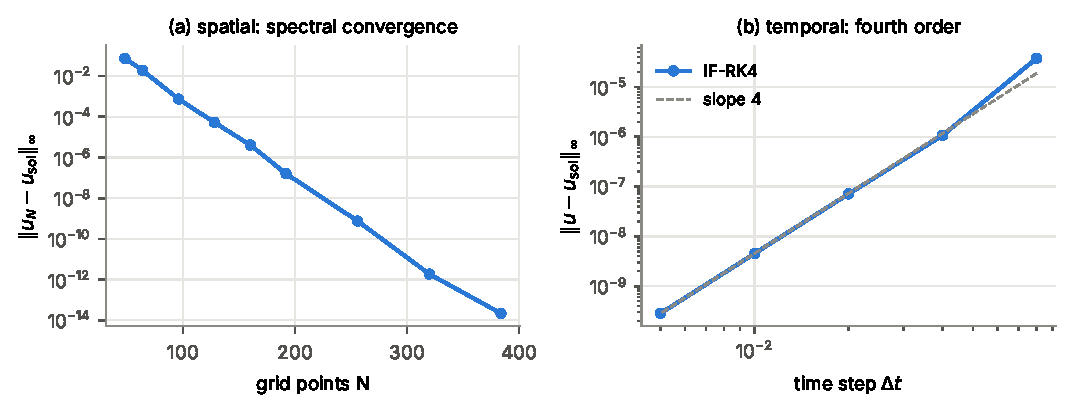
\includegraphics[width=\linewidth]{fig_convergence.pdf}
\caption{Verification of the KdV solver against the exact soliton.
(a) Spectral convergence with the number of grid points $N$.
(b) Fourth-order convergence with the time step $\Delta t$; the dashed line
has slope 4.}
\label{fig:convergence}
\end{figure}

\paragraph{Soliton interaction and conservation}
Fig.~\ref{fig:collision}a shows the overtaking collision of two solitons with
amplitudes 2 and 0.5 \cite{ZabuskyKruskal1965} ($N=512$, $L=150$,
$\Delta t=0.005$, $2\times10^4$ steps, about 4\,s). After the interaction
near $t\approx42$, both solitons re-emerge with amplitudes 2.0002 and
0.49999. Their measured phase shifts, $+2.698$ and $-5.3817$, agree with the
exact two-soliton values $\kappa_1^{-1}\ln[(\kappa_1+\kappa_2)/(\kappa_1-\kappa_2)]=+2.691$
and $-\kappa_2^{-1}\ln[(\kappa_1+\kappa_2)/(\kappa_1-\kappa_2)]=-5.3821$,
with $\kappa_j=\sqrt{\alpha A_j/12\beta}$ \cite{DrazinJohnson1989}, to within
0.3\% and 0.01\%. The remaining difference most likely arises because the initial
superposition of two solitons is not an exact two-soliton solution.
Over the whole run, the relative drift of the discrete mass stays
at round-off ($2.4\times10^{-16}$). The drifts of the $L^2$ norm and the
Hamiltonian, which IF-RK4 does not conserve exactly, reach
$5.6\times10^{-11}$ and $1.0\times10^{-10}$, respectively (Fig.~\ref{fig:collision}b).

\begin{figure}[t]
\centering
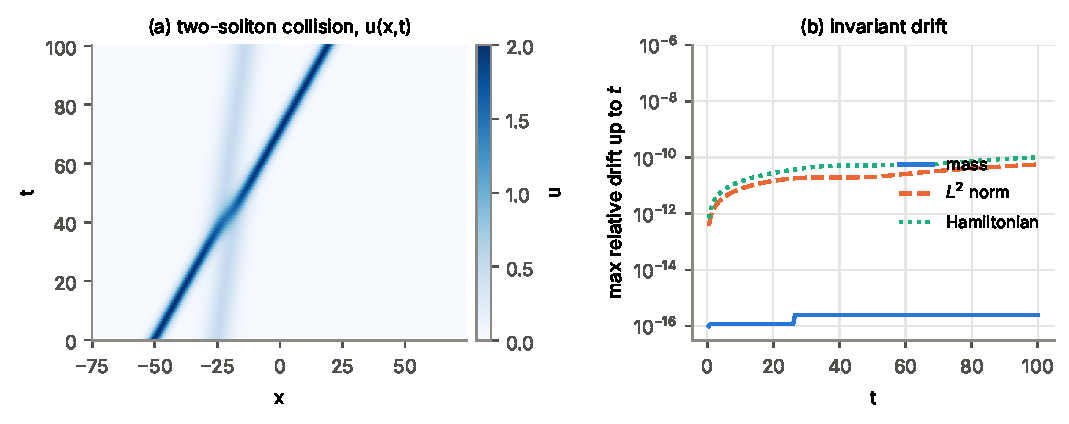
\includegraphics[width=\linewidth]{fig_collision.pdf}
\caption{(a) Space--time evolution of a two-soliton overtaking collision.
(b) Maximum relative drift of the discrete mass, $L^2$ norm and Hamiltonian up
to time $t$.}
\label{fig:collision}
\end{figure}

\begin{table}[t]
\centering\small
\caption{Summary of verification results, reproduced by
\texttt{examples/verification.py}. Each check also has a corresponding automated
test, which runs a shorter version of the computation.}
\label{tab:verification}
\begin{tabular}{@{}lll@{}}
\toprule
Check & Reference & Result \\
\midrule
Critical Mach number & Eq.~(\ref{eq:mc}) & $M_c=1.5852010652$ \\
Amplitude at $M=1.2$ & -- & $\phi_m=0.5243854849$ \\
Small-amplitude limit & KdV soliton & error $\propto\delta^{0.96}$ \\
Spatial convergence & exact soliton & $2.2\times10^{-14}$ at $N=384$ \\
Temporal convergence & exact soliton & observed order 3.99 \\
Collision phase shifts & $+2.691$, $-5.382$ & $+2.698$, $-5.382$ \\
Mass drift ($2\times10^4$ steps) & conserved & $2.4\times10^{-16}$ \\
Hamiltonian drift & conserved & $1.0\times10^{-10}$ \\
\bottomrule
\end{tabular}
\end{table}

%% ------------------------------------------------------------------
\section{Impact}
\label{sec:impact}

PlasmaWaveLab is not intended to contribute new plasma theory. Its contribution
is a verified, citable reference implementation of two of the most widely used
calculations in nonlinear plasma-wave research. It is expected to be useful in
three ways.

\emph{Verification of new results.} Most Sagdeev and KdV studies extend the
cold-ion/Boltzmann-electron model by adding species (dust grains, positrons,
negative ions) or non-Maxwellian electron distributions. Each such extension
must reduce to the classical model in the appropriate limit. PlasmaWaveLab
provides that limit with documented tolerances. Its value of $M_c$, its
amplitudes and its profiles can therefore serve as regression targets for
new codes, and the explicit Sagdeev--KdV bridge shows how to quantify the
validity of a reduced model instead of assuming it.

\emph{Reproducibility.} Every number in this paper is regenerated by one
command and stored together with the software versions. Grid sizes, domain lengths, time steps and the
main solver tolerances are function arguments with documented defaults. This
reproducibility is often missing from soliton studies in the literature.

\emph{Teaching.} The package is small enough to be read in full. It connects
the pseudo-particle picture, asymptotic reduction and spectral methods in a
single example, and so supports courses in plasma physics, nonlinear waves and
numerical analysis. Students can explore the existence domain or soliton
collisions from the command line without writing numerical code.

The pure-function design of the core makes it straightforward to add new
pseudopotentials or KdV-type models (for example, modified KdV or
Gardner equations) while keeping the existing tests as regression checks. The
author will use the package as the reference implementation for forthcoming work
on multi-species plasmas in the FIZMAKO group.

\paragraph{Limitations} The current release is restricted to one-dimensional,
unmagnetised, collisionless plasmas with cold ions and Boltzmann electrons, and
to positive-polarity solitons. Kinetic effects, finite ion temperature,
magnetic fields, multi-dimensional geometries and continuation through
double-layer or supersoliton regimes are not implemented. The KdV solver uses
periodic boundaries, so the domain must be wide enough to contain the soliton
tails.

%% ------------------------------------------------------------------
\section{Conclusions}
\label{sec:conclusions}

PlasmaWaveLab provides compact, tested and documented Python implementations of
the Sagdeev pseudopotential method and of a spectral IF-RK4 solver for the KdV
equation for ion-acoustic solitary waves. The two solvers are linked through
their explicit asymptotic relation. Spectral accuracy in space, fourth-order
accuracy in time, conservation to round-off or near round-off, the correct
critical Mach number, first-order agreement with the KdV limit and the exact
two-soliton phase shifts have all been demonstrated, and each is covered by an automated test that runs in continuous
integration. Planned developments
include multi-species and non-thermal pseudopotentials, negative-polarity
branches and double layers, and modified KdV and Gardner solvers.

%% ------------------------------------------------------------------
\section*{CRediT authorship contribution statement}
\textbf{Alvaro H. Salas:} Conceptualization, Methodology, Software, Validation,
Formal analysis, Visualization, Writing -- original draft, Writing -- review \& editing.

\section*{Declaration of competing interest}
The author declares that he has no known competing financial interests or
personal relationships that could have appeared to influence the work reported
in this paper.

\section*{Declaration of generative AI and AI-assisted technologies in the manuscript preparation process}
During the preparation of this work the author used Claude (Anthropic) to assist
with code refactoring, test design and language editing. After using this tool,
the author reviewed and edited the content as needed and takes full
responsibility for the content of the published article.

\section*{Acknowledgements}
The author thanks Universidad Nacional de Colombia, Sede Manizales, for its
institutional support.

%% ------------------------------------------------------------------
\begin{thebibliography}{99}

\bibitem{Sagdeev1966}
R.~Z. Sagdeev, Cooperative phenomena and shock waves in collisionless plasmas,
in: M.~A. Leontovich (Ed.), Reviews of Plasma Physics, Vol.~4, Consultants
Bureau, New York, 1966, pp. 23--91.

\bibitem{WashimiTaniuti1966}
H.~Washimi, T.~Taniuti, Propagation of ion-acoustic solitary waves of small
amplitude, Phys. Rev. Lett. 17 (1966) 996--998.
\doi{10.1103/PhysRevLett.17.996}.

\bibitem{Ikezi1970}
H.~Ikezi, R.~J. Taylor, D.~R. Baker, Formation and interaction of ion-acoustic
solitions [sic], Phys. Rev. Lett. 25 (1970) 11--14.
\doi{10.1103/PhysRevLett.25.11}.

\bibitem{Chen2016}
F.~F. Chen, Introduction to Plasma Physics and Controlled Fusion, 3rd ed.,
Springer, Cham, 2016. \doi{10.1007/978-3-319-22309-4}.

\bibitem{Korteweg1895}
D.~J. Korteweg, G.~de~Vries, On the change of form of long waves advancing in a
rectangular canal, and on a new type of long stationary waves, Philos. Mag. 39
(1895) 422--443. \doi{10.1080/14786449508620739}.

\bibitem{ZabuskyKruskal1965}
N.~J. Zabusky, M.~D. Kruskal, Interaction of ``solitons'' in a collisionless
plasma and the recurrence of initial states, Phys. Rev. Lett. 15 (1965)
240--243. \doi{10.1103/PhysRevLett.15.240}.

\bibitem{DrazinJohnson1989}
P.~G. Drazin, R.~S. Johnson, Solitons: An Introduction, Cambridge University
Press, Cambridge, 1989. \doi{10.1017/CBO9781139172059}.

\bibitem{Burns2020}
K.~J. Burns, G.~M. Vasil, J.~S. Oishi, D.~Lecoanet, B.~P. Brown, Dedalus: A
flexible framework for numerical simulations with spectral methods, Phys. Rev.
Res. 2 (2020) 023068. \doi{10.1103/PhysRevResearch.2.023068}.

\bibitem{Brent1973}
R.~P. Brent, Algorithms for Minimization without Derivatives, Prentice-Hall,
Englewood Cliffs, NJ, 1973.

\bibitem{DormandPrince1980}
J.~R. Dormand, P.~J. Prince, A family of embedded Runge--Kutta formulae,
J. Comput. Appl. Math. 6 (1980) 19--26. \doi{10.1016/0771-050X(80)90013-3}.

\bibitem{FornbergWhitham1978}
B.~Fornberg, G.~B. Whitham, A numerical and theoretical study of certain
nonlinear wave phenomena, Philos. Trans. R. Soc. Lond. A 289 (1978) 373--404.
\doi{10.1098/rsta.1978.0064}.

\bibitem{Trefethen2000}
L.~N. Trefethen, Spectral Methods in MATLAB, SIAM, Philadelphia, 2000.
\doi{10.1137/1.9780898719598}.

\bibitem{Orszag1971}
S.~A. Orszag, On the elimination of aliasing in finite-difference schemes by
filtering high-wavenumber components, J. Atmos. Sci. 28 (1971) 1074.
\href{https://doi.org/10.1175/1520-0469(1971)028\%3C1074:OTEOAI\%3E2.0.CO;2}{doi:\nolinkurl{10.1175/1520-0469(1971)028<1074:OTEOAI>2.0.CO;2}}.

\bibitem{CoxMatthews2002}
S.~M. Cox, P.~C. Matthews, Exponential time differencing for stiff systems,
J. Comput. Phys. 176 (2002) 430--455. \doi{10.1006/jcph.2002.6995}.

\bibitem{KassamTrefethen2005}
A.-K. Kassam, L.~N. Trefethen, Fourth-order time-stepping for stiff PDEs,
SIAM J. Sci. Comput. 26 (2005) 1214--1233. \doi{10.1137/S1064827502410633}.

\bibitem{Harris2020}
C.~R. Harris, K.~J. Millman, S.~J. van~der Walt, et~al., Array programming with
NumPy, Nature 585 (2020) 357--362. \doi{10.1038/s41586-020-2649-2}.

\bibitem{Virtanen2020}
P.~Virtanen, R.~Gommers, T.~E. Oliphant, et~al., SciPy 1.0: Fundamental
algorithms for scientific computing in Python, Nat. Methods 17 (2020) 261--272.
\doi{10.1038/s41592-019-0686-2}.

\bibitem{Hunter2007}
J.~D. Hunter, Matplotlib: A 2D graphics environment, Comput. Sci. Eng. 9 (2007)
90--95. \doi{10.1109/MCSE.2007.55}.

\end{thebibliography}

\end{document}
